
\clearpage

\newcommand{\highlight}[1]{{\color{BrickRed}\textbf{#1}}}

\section{Power Inputs for the Endcap Petal Model}

Table~\ref{tab:power_numbers} details the current, voltage, and power specifications for each
front-end component. The values should match the numbers used in the barrel thermal model.

\def\tid{\ensuremath{^*\xspace}}
\def\eff{\ensuremath{\varepsilon}}
\def\pfeast{\ensuremath{\frac{(1-\eff)}{\eff}(P_\text{ABC}+P_\text{HCC})}}
%
\let\arraystretcha\arraystretch
\renewcommand\arraystretch{1.2} % 1.6
\begin{table}[h!]
\begin{center}
\adjustbox{max width=\textwidth}{ %% just before tabular
\begin{tabular}{|l|c|c|c|c|c|c|c|} \hline
\multirow{2}{*}{Description} & input voltage & \multicolumn{4}{c|}{Specifications for 1 component} & $n$ components & Total power \\
              & [V]           & current [A] &\% bumped & power [W]                   & eff   & per module (1 side) & (1 side) [W] \\ \hline
AMAC 1.5V     & 1.5           & 0.042               &  & 0.063                       &       & --                  &       \\
AMAC 2.5V     & 2.5           & 0.002               &  & 0.005                       &       & --                  &       \\
Total AMAC    & --            & --                  &  & \color{blue}{0.068}         &       & R3: 2               & 0.136 \\
              &               &                     &  &                             &       & All others: 1       & 0.068 \\ \hline
ABC (digital) & 1.5           & 0.027          & 110\% & 0.0405                      &       & --                  &       \\
ABC (analog)  & 1.5           & 0.068               &  & 0.102                       &       & --                  &       \\
Total ABC     & --            & 0.095               &  & \color{blue}{0.1425}\tid    &       & R0: 17              & 2.423 \\
              &               &                     &  &                             &       & R1: 21              & 2.993 \\
              &               &                     &  &                             &       & R2: 12              & 1.710 \\
              &               &                     &  &                             &       & R3: 28              & 3.990 \\
              &               &                     &  &                             &       & R4: 16              & 2.280 \\
              &               &                     &  &                             &       & R5: 18              & 2.565 \\ \hline
HCC (digital) & 1.5           & 0.210         & 25.5\% & 0.315                       &       & --                  &       \\
HCC (analog)  & 1.5           & 0.0                 &  & 0.0                         &       & --                  &       \\
Total HCC     & --            & 0.210               &  & \color{blue}{0.315}\tid     &       & R3: 4               & 1.260 \\
              &               &                     &  &                             &       & All others: 2       & 0.630 \\ \hline
bPOL12V (ABC,HCC,AMAC1.5) & --&                     &  & \pfeast   \tid              & 72\%  & --                  & R0: \color{blue}{1.187} \\
              &               &                     &  &                             &       &                     & R1: \color{blue}{1.409} \\
              &               &                     &  &                             &       &                     & R2: \color{blue}{0.910} \\
              &               &                     &  &                             &       &                     & R3: \color{blue}{1.021+1.021} \\
              &               &                     &  &                             &       &                     & R4: \color{blue}{1.132} \\
              &               &                     &  &                             &       &                     & R5: \color{blue}{1.243} \\ \hline
linPOL12V (for AMAC2.5) & --  &                     &  & see text                    &       & --                  & R3: \color{blue}{0.450 + 0.450} \\
              &               &                     &  &                             &       & --                  & All others: \color{blue}{0.450} \\ \hline
Total Module  & --            &                     &  & \tid                        &       &                     & R0: 4.758 \\
              &               &                     &  &                             &       &                     & R1: 5.549 \\
              &               &                     &  &                             &       &                     & R2: 3.768 \\
              &               &                     &  &                             &       &                     & R3: 8.328 \\
              &               &                     &  &                             &       &                     & R4: 4.560 \\
              &               &                     &  &                             &       &                     & R5: 4.956 \\ \hline
\multicolumn{8}{|c|}{} \\[-2mm]
\multicolumn{8}{|c|}{EOS} \\ \hline
lpGBT                     & 1.2         & 0.317     &  & 0.380                       &       & --                  & \color{blue}{0.380} \\ \hline
VTRx (VL+) GBLD 1.2V      & 1.2         & 0.025     &  & 0.030                       &       & --                  & \\
VTRx (VL+) GBLD 2.5V      & 2.5         & 0.07      &  & 0.175                       &       & --                  & \\
VTRx (VL+) GBTIA (legacy) & 2.5         & 0.053     &  & 0.133                       &       & 1                   & \\
Total VTRx (VL+)          &             &           &  & 0.338                       &       & 1                   & \color{blue}{0.338} \\ \hline
bPOL2V5 (old DCDC2)       &             &           &  &                             & 88\%  & 2$\times$, master only         & \color{blue}{0.056+0.056} \\
bPOL12V       &               &                     &  &                             & 55\%  & 2$\times$, master only         & \color{blue}{0.633+0.633} \\ \hline
EOS Master    &               &                     &  &                             &       &                     & 2.096 \\
EOS Slave     &               &                     &  &                             &       &                     & 0.718 \\
EOS both sides&               &                     &  &                             &       &                     & 2.814 \\
\hline \end{tabular}
} %% resizebox after tabular
\end{center}
\caption{Endcap module inputs.
Values with \tid~next to them are affected by the TID bump in one way or another. The bPOL12V efficiency
is representative only; in reality it is temperature- and current-dependent.
Note that there are two bPOL12V converters and two linPOL12V converters on R3.
Further notes are
described in the text.
}
\label{tab:power_numbers}
\end{table}
\let\arraystretch\arraystretcha

Some notes on the numbers in the table:
\begin{itemize}
\item HCC and ABC power numbers correspond to unirradiated values.
\item Items marked with a ``\tid'' are affected by the digital current increase caused by the TID.
The bPOL12V is affected by the TID bump insofar as its power is determined by the ABC and HCC.
%% \item In the ABC, we have 42.5~mA digital with a 69\% bump, plus 70~mA analog. This is equivalent to
%% 29~mA fully bumped, and 83~mA non-bumped current. (Old values.)
\item The HCC is assumed to have a smaller TID bump than the ABC. This is accounted by an additional
scaling for the HCC case - see Section~\ref{tid_parameterization_details}. But because this scaling
is functionally the same as the ABC bump fraction, we write it here as well.
\item In the above, the bPOL12V efficiency is assumed to be constant, but in reality it is temperature- and
current-dependent.
\item In the EOS, the bPOL12V has a lower efficiency than in the module because the current load is
much smaller, and the bPOL12V is much less efficient in this regime.
\item The total module power (before irradiation, before TID bump) in the table represents
all components excluding HV and tape losses, which are small in comparison.
\end{itemize}

\noindent
Comments on the EOS components:

\begin{itemize}
%% \item For the EOS, the total power for both sides is simply double the power of one side.
\item The EOS bPOL12Vs and bPOL2V5s (was DCDC2) exist on one side only, and power the EOS cards on both petal
sides. There are two of each (one per side). Therefore the EOS numbers are split into ``master'' and ``slave'' numbers.
%% \item For $n=1$ lpGBTx ASICs (corresponding to the barrel long strips and the endcaps),
%% and assuming a BPOL12V efficiency $\varepsilon_\text{BPOL12V}=0.75$,
%% the total power is 1.4~W per EOS side.
%% \item For $n=2$ lpGBTx ASICs (corresponding to the barrel short strips), the total power is 2.6~W per
%% EOS side.
\end{itemize}

%% \subsection{The End-of-Substructure (EOS)}
%% \begin{itemize}
%% \item DCDC2 converter: $P=0.208$~W (see calculation below)
%% \item BPOL12V: $P=1.12$~W (see calculation below)
%% \item VTRx
%%   \begin{itemize}
%%     \item GBTIA: $I=53$~mA; 2.5~V; $P=0.1325$~W
%%     \item GBLD$_{2.5V}$: $I=18$~mA 2.5~V; $P=0.045$~W
%%   \end{itemize}
%% \item lpGBTx: $I=625$~mA; 1.2~V; $P=0.75$~W; powered by DCDC2
%% \item GBLD$_{1.2V}$: $I=9.5$~mA; 1.2~V; $P=0.0114$~W; powered by DCDC2
%% \end{itemize}

\subsection{Power Equations for the EOS, bPOL12V, bPOL2V5 and linPOL12V}

The total power of the EOS (one side) is given by:
\begin{equation}
P_\text{EOS} = \frac{1}{\varepsilon_\text{bPOL12V}}\times
  \left( \frac{1}{\varepsilon_\text{bPOL2V5}} (n P_\text{lpGBTx} + n P_\text{GBLD1.2}) + n P_\text{GBLD2.5} + P_\text{GBTIA} \right)
\end{equation}
% (((.750*2+0.0114*2)/0.88)+0.1325+0.045*2)/0.75 = 2.60
% (((.750*1+0.0114*1)/0.88)+0.1325+0.045*1)/0.75 = 1.40

As can probably be inferred from above, the power attributed to the EOS bPOL12V is:
\begin{equation}
P^\text{EOS}_\text{bPOL12V} = \frac{(1-\varepsilon_\text{bPOL12V})}{\varepsilon_\text{bPOL12V}}\times
  \left( \frac{1}{\varepsilon_\text{bPOL2V5}} (n P_\text{lpGBTx} + n P_\text{GBLD1.2}) + n P_\text{GBLD2.5} + P_\text{GBTIA} \right)
\end{equation}

The power in the EOS bPOL2V5 (was called DCDC2) converter is:
\begin{equation}
P^\text{EOS}_\text{bPOL2V5} = \frac{(1-\varepsilon_\text{bPOL2V5})}{\varepsilon_\text{bPOL2V5}} \left(n P_\text{lpGBTx} + n P_\text{GBLD1.2}\right)
\end{equation}


The power dissipated by the linPOL12V (powering the AMAC) is given by the current in the AMAC components
(adding the quiescent current, 1.9 mA) multiplied by the voltage drop in the linPOL12V:
\begin{equation}
P_\text{linPOL12V} = (I^{1.5V}_\text{AMAC} + I^\text{q}_\text{linPOL12V})\left(  \Delta V_\text{linPOL12V} - 1.5V \right)
                   + (I^{3.0V}_\text{AMAC} + I^\text{q}_\text{linPOL12V})\left(  \Delta V_\text{linPOL12V} - 3.0V \right)
\label{eq:amac_regulator}
\end{equation}
where the calculation of $\Delta V_\text{linPOL12V}$ is described in Section~\ref{low_voltage}.

\subsection{bPOL12V (FEAST) efficiency}

The bPOL12V efficiency varies as a function of temperature and load current. The parameterization used
is the one derived by Georg. Figure~\ref{feast_vs_temperature} highlights the agreement between the
measured FEAST efficiencies and the parameterized fit.

\begin{figure}[ht!]
\begin{center}
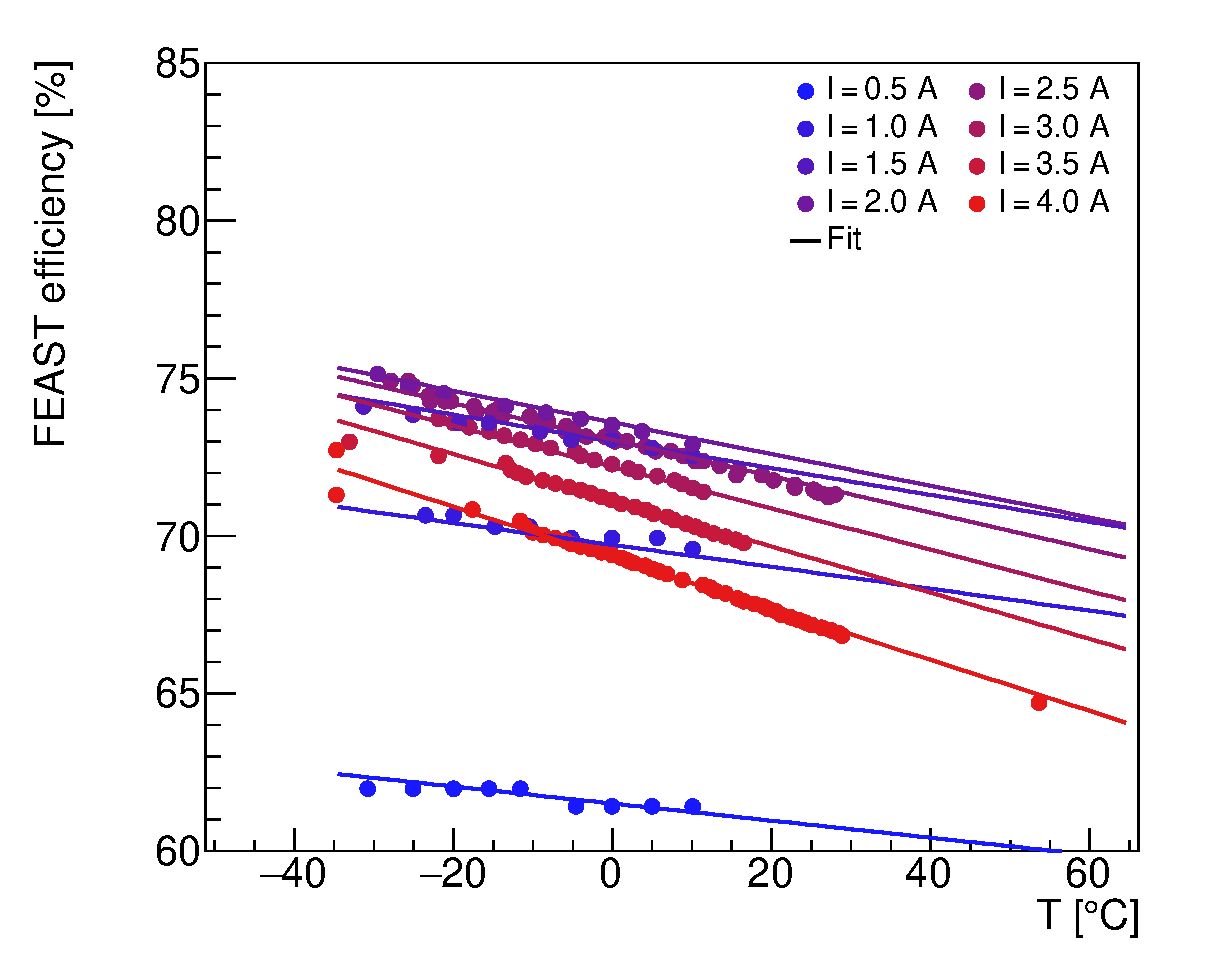
\includegraphics[width=0.49\linewidth]{figures/FeastEfficiency_isoCurrent}
\end{center}
\caption{FEAST efficiency data versus temperature ($x$-axis) and current (indicated with different
colors). The parameterization of the data is represented by the fit lines at fixed current.
}
\label{feast_vs_temperature}
\end{figure}

\subsection{TID bump parameterization}
\label{tid_parameterization_details}

The TID bump parameterization is the one supplied by Kyle Cormier for the ABC130$^{*}$
(Nominal parameters: $a=1.402\times 10^{11}$, $b=-1.62$.
Pessimistic parameters: $a=2.64\times10^{9}$, $b=-1.35$.)
Figure~\ref{tid_parameterization} shows the TID parameterization used in the current model. This
parameterized bump is applied to the ``bumped'' fraction of digital current, as indicated in
Table~\ref{tab:power_numbers}.

\begin{figure}[ht!]
\begin{center}
\begin{subfigure}[t]{0.49\textwidth}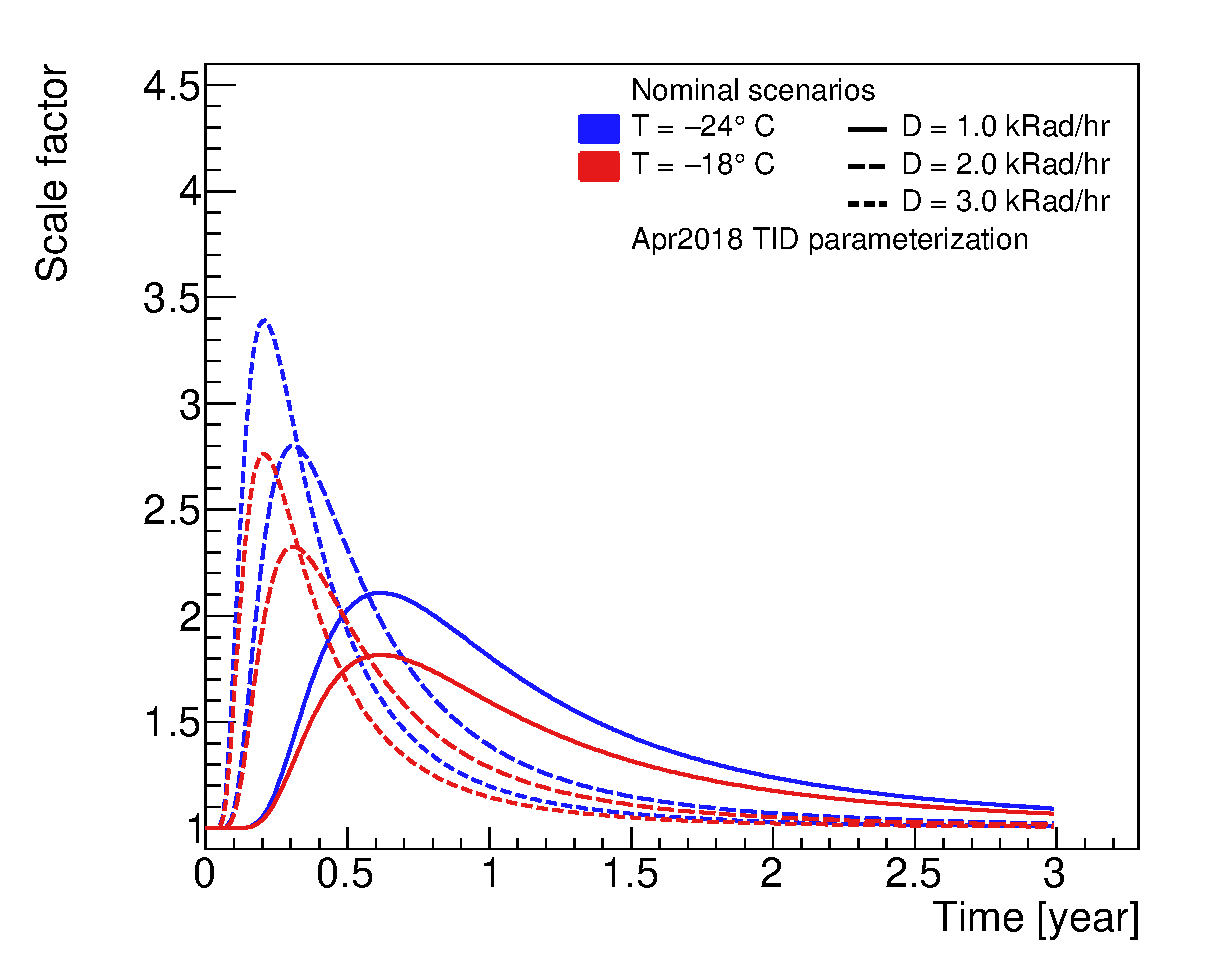
\includegraphics[width=0.99\linewidth]{figures/AbcTidBumpVersionRatesAndTemps_Nominal}\caption{Nominal Case}\end{subfigure}
\begin{subfigure}[t]{0.49\textwidth}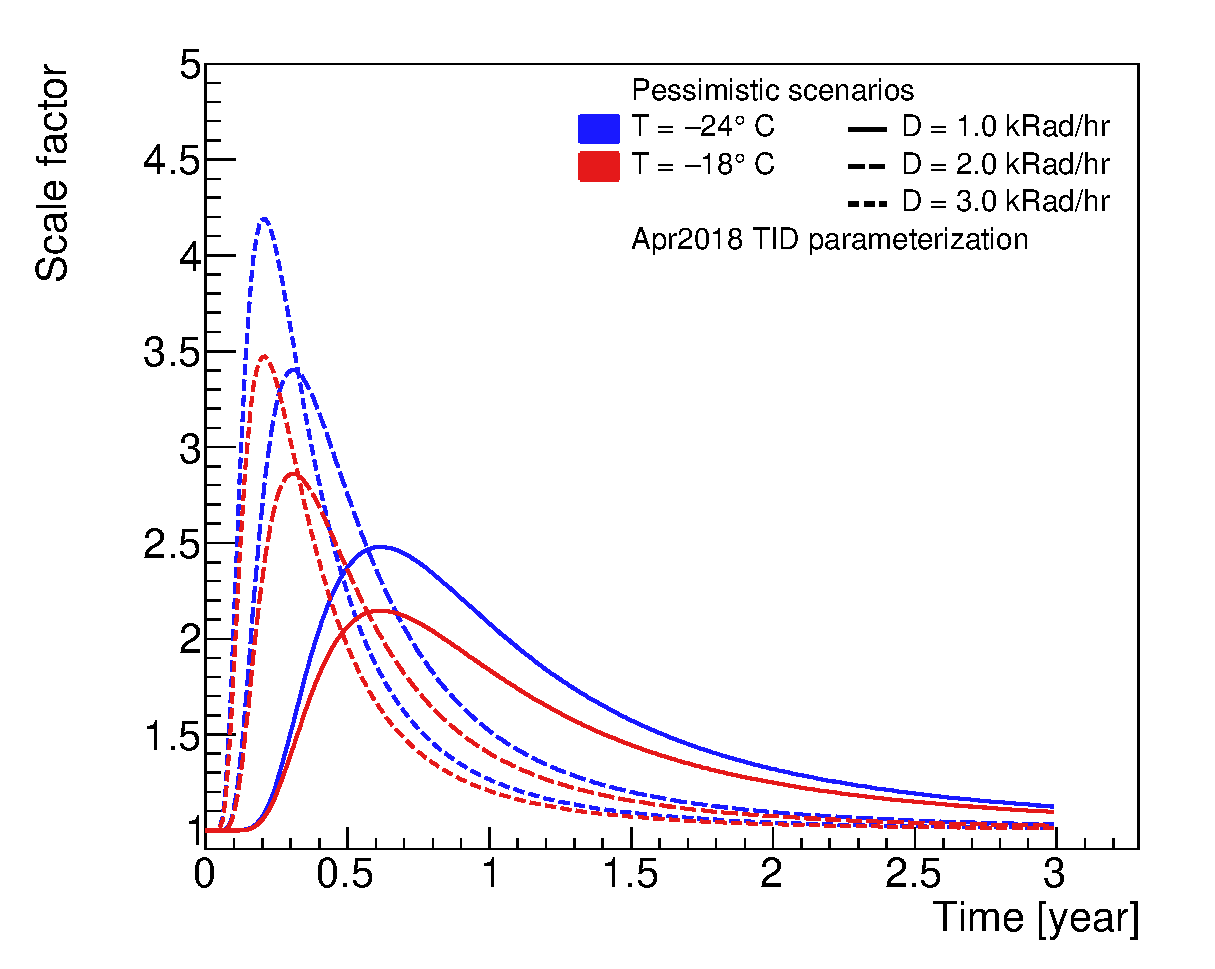
\includegraphics[width=0.99\linewidth]{figures/AbcTidBumpVersionRatesAndTemps_Pessimistic}\caption{Pessimistic Case}\end{subfigure}
\end{center}
\caption{TID parameterization vs time, for two representative temperatures (indicated by
color) and three dose rates (indicated by line style). Nominal and Pessimistic cases are shown.}
\label{tid_parameterization}
\end{figure}

\subsubsection*{HCC Treatment}

The HCC is assumed to have a smaller TID bump than the ABC. Thus, the HCC TID bump
is scaled by a factor (see Table~\ref{tab:power_numbers}) to account for the smaller observed HCC TID bump.

\subsection{Summary of Power Contributions in R1}

A stack plot showing the contributions of each component to the total power is shown in
Figure~\ref{power_stackplot}.

\begin{figure}[ht!]
\begin{center}
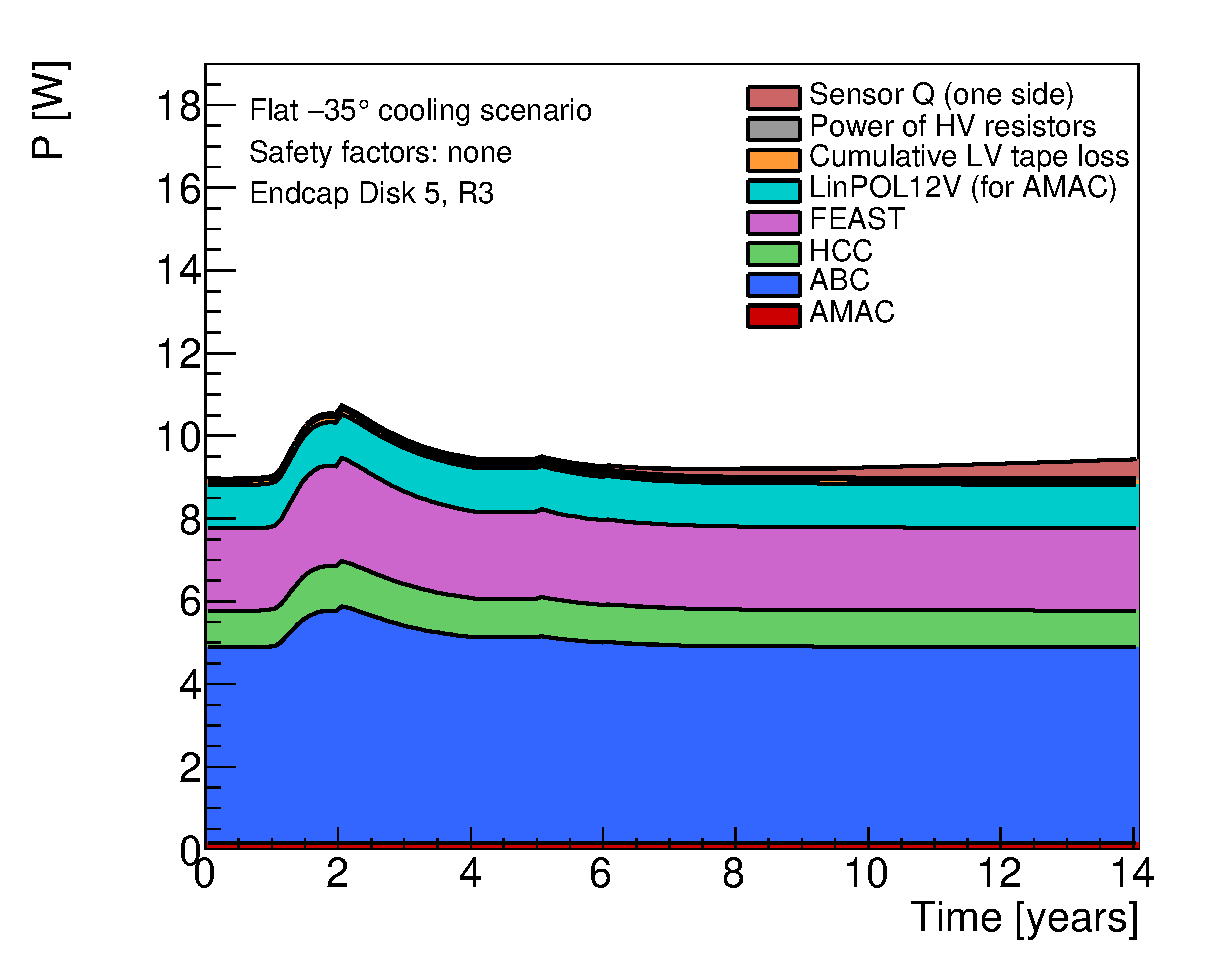
\includegraphics[width=0.55\linewidth]{figures/PowerStackPlot.eps}
\end{center}
\caption{Summary of the contributions of each front-end component to the total power in R3 (Disk 5), given
a nominal TID bump parameterization and no safety factors, to illustrate the relative contributions
of each component.}
\label{power_stackplot}
\end{figure}

